\section{3D exploration strategies}

In contrast to 2D exploration and mapping strategies, mapping of large environments in 3D requires high memory and
computational consumptions. 
Different autonomous 3D exploration strategies were proposed so that 2D
exploration tools are used to three dimensions. In \cite{Joho2007}, Joho et al. presented an exploration strategy that extends the known 2D exploration strategies into the 3D space. Mapping is done using multi-level surface maps while a cost function takes
into account an expected information gain and a travel cost. 
Bachrach et
al. \cite{Bachrach2009} presented a solution for enabling a quadrotor helicopter to
autonomously explore and map unstructured indoor environments. Authors useed a 2D frontier-based
exploration algorithm and set a fixed altitude for the helicopter
during exploration.  

Dornhege and Kleiner \cite{Dornhege2013} used a frontier based method extended to 3D exploration. This method requires high computational effort and operating environment is limited
to small workspaces. On the other hand, Maurovic et al. \cite{Maurovic2014} presented a 3D exploration strategy for a mobile
robot equipped with a 3D laser scanner. This strategy ensures an on-line room detection algorithm focused on the room-by-room exploration keeping the memory and computational
requirements low.

Next-best-view approach in the process of building 3D model of a real object used without any a priori information about the environment was described in \cite{VasquezGomez2014}. The algorithm determines each view to reconstruct an arbitrary object. Furthermore, authors proposed a method to deal with the uncertainty in sensor positioning.
Next-best-view approach for 3D exploration was presented by Bircher et. al. \cite{Bircher2016}. Authors presented a novel path planning algorithm for the autonomous exploration of an unknown area. The proposed planner finds the best branch in an on-line computed tree. The quality of the branch is determined by the amount of unmapped space that
can be explored. The planner is capable of running online, onboard a robot with limited resources.

Baiming et al. \cite{Baiming2018} presented a new target points based trajectory planning algorithm to explore unknown space. The proposed method progressively plans long-term
target point, intermediate target point, local target points,
and local trajectory within real time constraint. By tracking
 the trajectory, robot can efficiently explore the unknown space while avoiding obstacles.

Zhu
et al. \cite{Zhu2015} developed a vision-based tool that performs autonomous exploration using an MAV equipped with 3D sensors. A real time frontier based exploration strategy is
used to build maps that are stored in the OctoMap format (Fig. \ref{fig:octomap}).

\begin{figure}[t!]
	\centering
	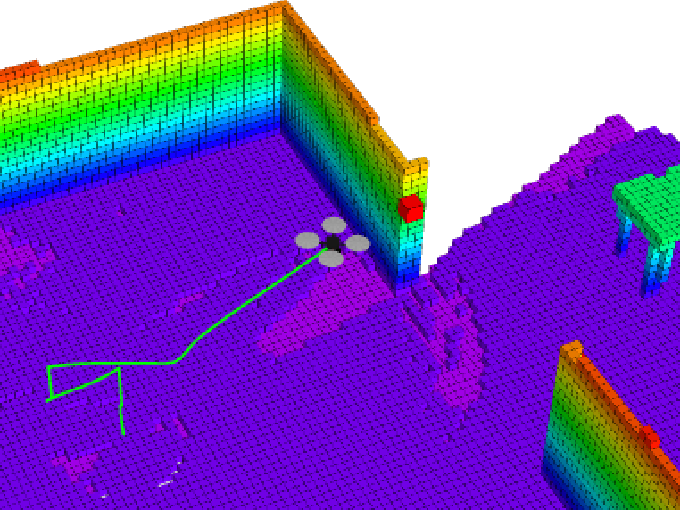
\includegraphics[width=1.0\columnwidth]{./pictures/octomap_and_drone.png}	
	\caption{UAV exploration in 3D environment. The colored voxels are 3D OctoMap representation and the green lines show the exploration trajectory \cite{Wang2019}.}
	\label{fig:octomap}
\end{figure}

Continuous cells are gathered into clusters and representative cells are chosen for each cluster. An
evaluation function is used to choose the best representative
cell and only state-changed space in the 3D map is processed
in each iteration.
Authors in \cite{Senarathne2016} presened an alternative approach to 3D
exploration based on surface frontier voxels. The strategy focuses on seeking the expansion of mapped surfaces, instead of reducing unmapped voxels. 

Vutetakis in \cite{Vutetakis2019} proposed a novel startegy for inspecting
critical infrastructure autonomously using Micro Aerial Vehicles (MAV). In order to facilitate
autonomous inspection capabilities, this strategy address the problem of autonomous MAV exploration and coverage of an unknown
structure to acquire the spatial information necessary for the
development of a high-fidelity 3D model of the structure. Key to
this problem is to not only cover the entire structure, but also to minimize
accumulative data errors during the exploration through direct
planning of loop closures. 

The 3D exploration problem using aerial vehicles within limited flight endurance was addressed by Wang et al. \cite{Wang2019}. Authors proposed an information potential field based method considering both the traveled cost and information-gain. The next-best-view point is chosen based on a
multi-objective function which considers information of several
candidate regions and the traveled path cost. The selected goal
attracts the robot while known obstacles form the repulsive
force repel the robot.

\begin{figure}[t!]
	\centering
	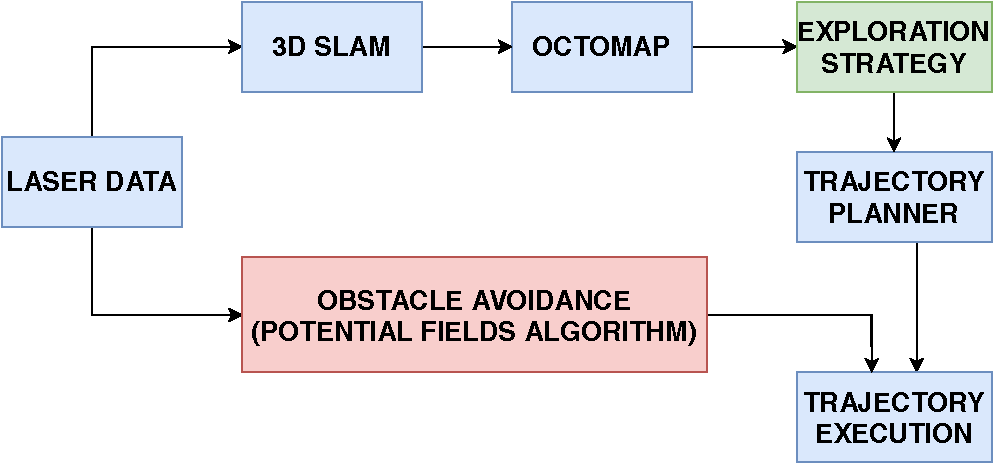
\includegraphics[width=1.0\columnwidth]{./pictures/3D_strategy.pdf}	
	\caption{Diagram of the implemented 3D exploration strategy.}
	\label{fig:3D_strategy}
\end{figure}
